\subsection{Lebensdauermessung}
Der Aufbau zur Lebensdauermessung ist in Abbildung \ref{fig:lebensdauer_aufbau} zu sehen. Fliegt ein Myon durch den ersten und in den zweiten Szintillationszähler löst es zwei Signale aus die zur Koinzidenz führen. Dies ist dann der Startimpuls der die Zeitmessung startet. Die Zeitmessung geschieht dabei durch das Zählen von Impulsen eines \SI{20}{\mega\hertz}-Oszillators. Zerfällt das Myon in dem zweiten Zähler löst es den Stopimpuls für die Zeitmessung aus. Damit das Startsignal nicht gleichzeitig auch das Stopsignal ist wird das Startsignal mit einem Verzögerungskabel verzögert. Fliegt ein Myon durch den zweiten Zähler ohne zu zerfallen wird kein Stopsignal ausgelöst.

\begin{figure}[h]
  \centering
  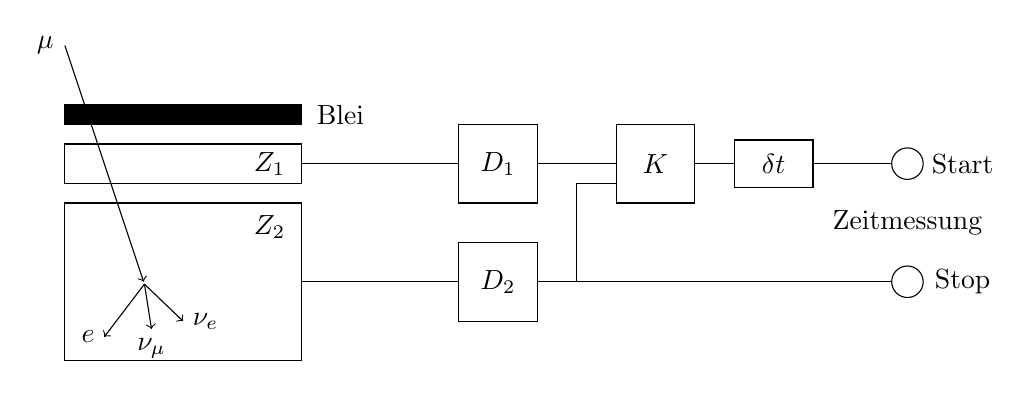
\begin{tikzpicture}
    \draw [fill=black] (0,5) rectangle (3,5.25);
    \draw (3.5,5.125) node {Blei};
    \draw (0,4.25) rectangle (3,4.75);
    \draw (2.6,4.5) node {$Z_1$};
    \draw (0,2) rectangle (3,4);
    \draw (2.6,3.7) node {$Z_2$};
    \draw (3,4.5)--(5,4.5);
    \draw (5,4) rectangle (6,5);
    \draw (5.5,4.5) node {$D_1$};
    \draw (6,4.5)--(7,4.5);
    \draw (7,4) rectangle (8,5);
    \draw (7.5,4.5) node {$K$};
    \draw (8,4.5)--(8.5,4.5);
    \draw (8.5,4.2) rectangle (9.5,4.8);
    \draw (9,4.5) node {$\delta t$};
    \draw (9.5,4.5)--(10.5,4.5);
    \draw (10.7,4.5) circle (0.2);
    \draw (11.4,4.5) node {Start};
    \draw (3,3)--(5,3);
    \draw (5,2.5) rectangle (6,3.5);
    \draw (5.5,3) node {$D_2$};
    \draw (6,3)--(6.5,3)--(6.5,4.25)--(7,4.25);
    \draw (6.5,3)--(10.5,3);
    \draw (10.7,3) circle (0.2);
    \draw (11.4,3) node {Stop};
    \draw (10.7,3.75) node {Zeitmessung};
    \draw [->] (0,6)--(1,3);
    \draw [->] (1.01,2.97)--(0.5,2.3) node [left] {$e$};
    \draw [->] (1.01,2.97)--(1.5,2.5) node [right] {$\nu_e$};
    \draw [->] (1.01,2.97)--(1.1,2.4) node [below] {$\nu_\mu$};
    \draw (-0.25,6) node {$\mu$};
  \end{tikzpicture}
  \caption{Versuchsaufbau zur Bestimmung der Lebensdauer von Myonen}
  \label{fig:lebensdauer_aufbau}
\end{figure}
